%%%%%%%%%%%%%%%%%%%%%%%%%%%%%%%%%%%%%%%%%%%%%%%%%%%%%%%%%%%%%%%%%%%%%%%%%%%
% Copyright (c) 2010 committers of YAKINDU and others.
% All rights reserved. This program and the accompanying materials
% are made available under the terms of the Eclipse Public License v1.0
% which accompanies this distribution, and is available at
% http://www.eclipse.org/legal/epl-v10.html
%
% Contributors:
%     committers of YAKINDU - initial API and implementation
%%%%%%%%%%%%%%%%%%%%%%%%%%%%%%%%%%%%%%%%%%%%%%%%%%%%%%%%%%%%%%%%%%%%%%%%%%%
\section{Example Scenario}

The example scenario is a simple pedestrian traffic light. A pedestrian can press
a button to indicate, she/he wants to cross the street. Then a blinking white
light indicates, that the traffic light has recognized the request. After a few
seconds, the traffic light for the street turns to red and the pedestrian traffic
light turns to green. Then the pedestrian traffic light turns to red and the
street traffic light changes to green again.
    
The state machine to model this behaviour is shown on figure
\ref{fig:statemachine}. This state machine must not be created but is shipped
with the example project and can be found in the
\texttt{workspace/Traffic\_Light/} directory.
    
\begin{figure}[ht] \center
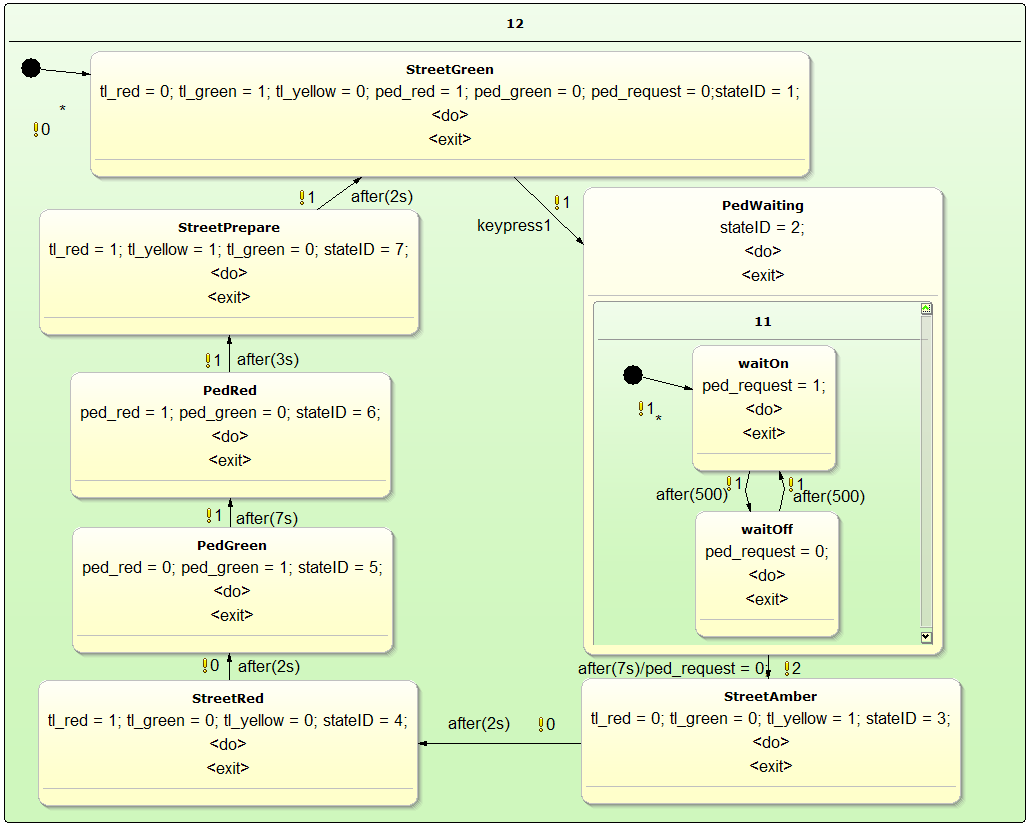
\includegraphics[width=0.8\textwidth]{./Pictures/Statemachine}
\caption{\label{fig:statemachine}Statemachine for the Traffic Light Example}
\end{figure}

% The embedded system that is used with this scenario is a ATMega128 Controller
% on a Display3000 board. This system was extended by an additional board
% representing a traffic light controlled crossroad. This board is connected to
% the Display3000 board.

\section{Starting the workflow}

The source code is created by starting the MWE workflow. This workflow can be
found in the \textit{traffic light} example directory:

\begin{figure}[h!] \center
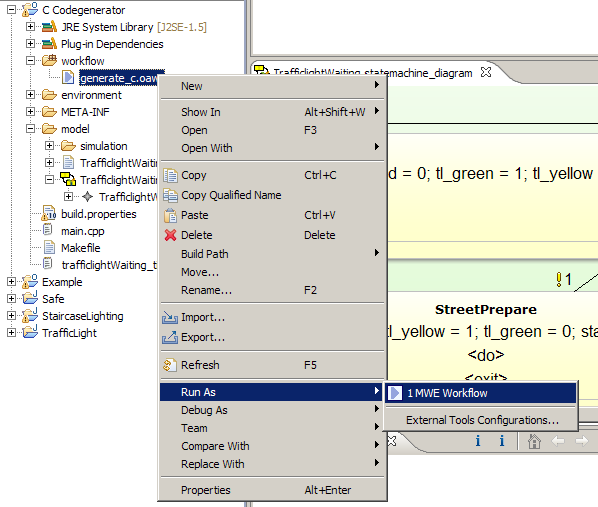
\includegraphics[width=0.8\textwidth]{./Pictures/workflow}
\caption{\label{fig:workflow}Starting the oAW-workflow to create the sources}
\end{figure}
\newpage

The generated C source code can be found within the new directory \texttt{c-src-gen}:

\begin{figure}[h!] \center
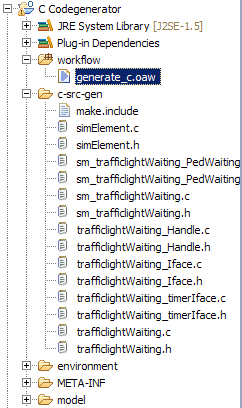
\includegraphics[width=0.3\textwidth]{./Pictures/sources}
\caption{\label{fig:sources}The sources are placed into the \textit{c-src-gen} directory}
\end{figure}

\newpage
%Hier fehlt noch was: wie wird der Workflow gestartet, und was muss alles vorhanden sein, damit der workflow tatsaechlich starten kann.
%-> Nutzer oAW
%-> Wo liegt das Ergebnis (Code)
%-> was kann man einstellen (Properties)

\section{Code Integration into an Existing Project}

Aside the source code for the state machine and the code for the interfaces, the
code generator creates a file called \texttt{make.include}. This file can easily
be included into an existing makefile by the line:

\begin{verbatim}
include c-src-gen/make.include
\end{verbatim}

The files, which are needed for the compilation, are added to the environment
variable \texttt{SM\_SOURCE}, so you have to add these sources to your project
sources:

\begin{verbatim}
OBJECTS    = main.o $(ENV_OBJ) $(GRAPHIC_OBJ) $(SM_SOURCE)
\end{verbatim}
%$

Additionally you should add the \texttt{c-src-gen} directory to the include and
source paths, so that the headers and sources could be found.
 
The example is designed for the Display3000 board, so the \textbf{Makefile} was
designed to create a binary for this hardware. Therefor it requires the AVR-gcc
toolchain to be able to compile. The toolchain contains a compiler, a linker and
some other usefull tools e.g. to download the data.

So go to your workspace directory with a shell and from there into the base
directory of your project and call \texttt{make}:

\begin{verbatim}
workspace$ cd Traffic_Light
Traffic_Light$ make
[...] compiling [...]
avr-gcc -Wall -Os -DF_CPU=7456000 -mmcu=atmega128 -I. -I./graphicLib [...]
rm -f main.hex
avr-objcopy -j .text -j .data -O ihex main.elf main.hex
\end{verbatim} 

If the compile was successful, you have a working binary \texttt{main.hex} that
could be deployed on the target.

To transfer the binary, you can use \texttt{make flash}.

\section{State Machine Access}

As mentioned before, the code for the state machine can be found in the folder
\textbf{c-src-gen}. After running the workflow the following files should be
available in this directory:

\begin{verbatim}
c-src-gen$ ls
make.include                        sm_trafficlightWaiting_PedWaiting.h
simElement.c                        trafficlightWaiting.c
simElement.h                        trafficlightWaiting.h
sm_trafficlightWaiting.c            trafficlightWaiting_Iface.c
sm_trafficlightWaiting.h            trafficlightWaiting_Iface.h
sm_trafficlightWaiting_Handle.c     trafficlightWaiting_timerIface.c
sm_trafficlightWaiting_Handle.h     trafficlightWaiting_timerIface.h
sm_trafficlightWaiting_PedWaiting.c
\end{verbatim}
% $

The files completely define the state machine. How to integrate the source into
another project, was subject of the previous section.

The files \texttt{sm\_trafficlightWaiting.*} and
\texttt{sm\_trafficlightWaiting\_PedWaiting.*} represents the two regions in the
state chart. The header- and C-file called
\texttt{sm\_trafficlightWaiting\_Handle.*} contain the main handle, which is
called \texttt{SM\_trafficlightWaiting\_Handle}. Please do not access the state
machine handle information directly.

The structure carries the information about the current state, the actual
transition, that has been activated, the handle for the first level region and
the interface handle. The handle is initialized with the function
\texttt{trafficlightWaiting\_init(\&sMachineHandle, \&interfaceHandle)}. Here the
\texttt{sMachineHandle} is the state machine handle and the
\texttt{interfaceHandle} is a \underline{pointer} to an interface handle. The
initialization call initializes the whole state machine and returns the interface
handle pointer.

For convenience all a state machine user needs to include is
\texttt{trafficlightWaiting.h}. This header includes all other necessary
information.
 
\section{Operating System and Drivers for the Example Device}

To let the state machine run on the Display 3000 development board, the system
needs a minimal \textbf{operating system} (OS) and some drivers for input and
output. This operating system is found in the \texttt{environment} directory.
This cooperative OS is written in C++ and contains an input driver for the 6 keys
on the hardware board and an output driver for the display and a LED board that
is connected to the \textit{port A}.

Because of copyright restrictions, the display driver is not included into this
example. The calls to the display interface can included by adding
\texttt{-DWITH\_DP3000\_GL} to the compiler options and updating the include
path defined in variable \texttt{COMPILETT} of the Makefile to point to the
right AVR-Libraries.

The transfer of the LED data uses a simple software driven SPI-like interface
with three connections (data, clock and inherit).

The rest, like shifting the data, is done by the hardware board.

Following files belong to the operating system:
\begin{verbatim}
definitions.h  event.h      scheduler.cpp  task.cpp
event.cpp      prioQueue.h  scheduler.h    task.h
\end{verbatim}

The \texttt{key*} files contain the driver for a debounced key input. The
\texttt{output*} files contain the driver code to create the output. To create
the cycles for the state machine, this behaviour is placed in the files
\texttt{statemachine*}.

\begin{figure}[h!]
\center
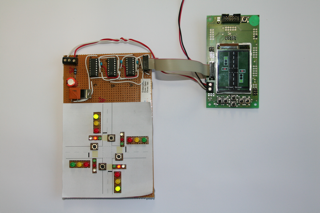
\includegraphics[width=0.8\textwidth]{./Pictures/Board1}
\caption{\label{fig:board1}Display3000 Development board with additional Hardware}
\end{figure}

After generation of source code by the workflow, it is possible to call the
Makefile inside the root directory of this example. By default this File calls
the commands \textbf{avr-gcc} and \textbf{avr-g++}. If you like to send
the binary to the micro controller, it is neccessary to check the \texttt{PORT}
variable inside the Makefile and \textbf{avrdude} needs to be on classpath. If
everything is correct, \texttt{make flash} will send the binary to the controller.
\newpage

